\documentclass{article}
\usepackage[UTF8]{ctex}
\usepackage[tc]{titlepic}
\usepackage{titlesec}
\usepackage{cite}
\usepackage{amsmath}
\usepackage{amsfonts}
\usepackage{fancyhdr}
\usepackage{booktabs}
\usepackage{graphicx}
\usepackage{geometry}
\usepackage{caption}
\usepackage[section]{placeins}
\geometry{a4paper,scale=0.8}
\pagestyle{fancy}

\lhead{第二次作业\\\today}
\chead{中国科学技术大学\\数学建模课程}

\rhead{Assignment x\\ {\CTEXoptions[today=old]\today}}
\newcommand{\upcite}[1]{\textsuperscript{\cite{#1}}}

\titleformat*{\section}{\bfseries\Large}
\titleformat*{\subsection}{\bfseries\large}

\title{\bfseries 基于矩阵SVD分解的图像压缩}
\author{时分 \quad  101 \quad  PB23151799}

\begin{document}
\maketitle
\begin{abstract}
    奇异值分解（SVD）是一种矩阵的分解方式，它可以将矩阵分解成若干矩阵的线性组合，系数越大的矩阵在原矩阵中就越关键。本报告介绍了一种简单的图像压缩方法，描述了基于矩阵SVD分解的数学建模原理。在MATLAB环境下针对灰度图像和RGB图像完成了代码实现，将其应用于示例图像的压缩。最后讨论了本算法的不足。
\end{abstract}
\clearpage
% \setcounter{secnumdepth}{1}
 \setcounter{section}{1}
\section*{\centerline{一、前言}}
    矩阵的奇异值分解（Singular Value Decomposition, SVD）是一种便捷的矩阵分解方法，能够发现数据中的一些潜在模式，常被应用于文本分析、推荐系统、金融数据分析、传感器数据压缩等任务中。\upcite{Man2017} 在计算机视觉和图像处理领域，图像通常被表示为标准的矩阵（即像素的数值排列），每个通道可以看作一个矩阵，或多个通道组合成一个三维张量，这种结构使得其天然适用于线性代数工具，如SVD、主成分分析（PCA）和傅立叶变换（FFT）等。其中，SVD分解可以应用于图像的存储优化（压缩）、图像传输、去噪、特征提取等任务。本报告介绍了基于SVD分解的简单图像压缩算法，其通过选取较大奇异值所对应的特征向量并重组来达成对图像的压缩操作，具有较好的效果和时间性能。

 \setcounter{section}{2}
\section*{\centerline{二、相关工作}}
    \subsection{图像压缩的技术背景}
    图像压缩的核心目标是减少存储和传输所需的数据量，同时尽可能保留视觉质量。传统方法包括有损压缩（如JPEG基于离散余弦变换）和无损压缩（如PNG基于预测编码）。近年来，基于矩阵分解的压缩方法因其数学理论严谨性受到关注，其中奇异值分解（SVD）因其对矩阵低秩逼近的优良性质，成为图像压缩的重要工具。
    \subsection{现有研究进展}
    已有研究表明，SVD在灰度图像压缩中能有效平衡压缩率与重构质量，但对彩色图像需分通道处理。部分研究结合SVD与小波变换，进一步提升压缩效率。然而，SVD的高计算复杂度（\(O(n^3)\)）限制了其在大规模图像中的应用，需通过截断策略优化计算成本。

 \setcounter{section}{3}
\section*{\centerline{三、问题分析}}
    将图像视为矩阵：灰度图像为二维矩阵\(\mathbf{A} \in \mathbb{R}^{m \times n}\)，彩色图像可分解为RGB三个通道矩阵。图像压缩问题转化为通过SVD寻找矩阵的低秩近似，使得存储量显著降低。
    
    特别地，对于RGB图像需要分通道独立压缩，之后再进行合成。

 \setcounter{section}{4}
\section*{\centerline{四、建模的假设}}
    本报告的实验基于以下假设：
    \begin{itemize}
      \item 假设图像矩阵的奇异值衰减较快，即前r个奇异值包含大部分能量，处理后能保留主要视觉信息。
      \item 对彩色图像，假设RGB三通道可独立进行SVD压缩，忽略通道间的相关性。
      \item 假设实验环境下SVD分解的计算资源（如内存、时间）可接受，暂不优化分解算法本身。
    \end{itemize}
 \setcounter{section}{5}
\section*{\centerline{五、符号说明}}
\begin{table}[h]
    \caption{\textbf{符号说明}}%标题
    \centering%把表居中
    \begin{tabular}{ccc}%内容全部居中
    \toprule%第一道横线
    符号&说明&单位 \\
    \midrule%第二道横线 
    $\mathbf{A}$ &图像矩阵 & / \\
    $\mathbf{U,\Sigma,V}$ & 奇异值分解矩阵 & / \\
    $\sigma_i$ & 奇异值 & / \\
    $r$ & 保留的奇异值个数（阶） & / \\
    \bottomrule%第三道横线
    \end{tabular}
\end{table}

 \setcounter{section}{6}
\section*{\centerline{六、数学模型建立}}
\subsection{SVD分解的数学模型}
    定义矩阵\(\mathbf{A} \in \mathbb{R}^{m \times n}\)的SVD为
    \[\mathbf{A} = \mathbf{U} \mathbf{\Sigma} \mathbf{V}^{T}\]
    其中\(\mathbf{U} \in \mathbb{R}^{m \times m}, \mathbf{V} \in \mathbb{R}^{n \times n}\)均为正交矩阵，\(\mathbf{\Sigma} \in \mathbb{R}^{m \times n}\)除了主对角线的元素以外全为0，主对角线上的元素即为奇异值。
    
    若将\(\mathbf{U},\mathbf{V}\)分别写为列向量的形式，即
    \[\mathbf{A} = \begin{pmatrix}
                     \mathbf{u}_1 & \mathbf{u}_2 & \dots & \mathbf{u}_m 
                   \end{pmatrix} \mathbf{\Sigma} \begin{pmatrix}
                                                   \mathbf{v}_1^T \\
                                                   \mathbf{v}_2^T \\
                                                   \vdots \\
                                                   \mathbf{v}_n^T
                                                 \end{pmatrix}\]
    则可以将\(\mathbf{A}\)分解为若干秩为1的矩阵的线性组合
    \[\mathbf{A} = \sigma_1 \mathbf{u}_1\mathbf{v}_1^T + \sigma_2 \mathbf{u}_2\mathbf{v}_2^T + \dots + \sigma_k \mathbf{u}_k\mathbf{v}_k^T\]
    其中\(\sigma_i\)是第i个奇异值，\(k = \min\{m,n\}\)。
    
    直观地看，\(\sigma_i\)越大的项保留了原矩阵中越重要的信息。在算法中，对图像（或其通道）的矩阵保留系数最大的前r个项，即可实现不同程度的图像压缩。\upcite{Jimbo2023} 
    
    在应用上，既可以选择保留的项的个数，也可以选择保留的能量信息比例。\upcite{iGEO2022} 常见的方法是先求得所有奇异值平方总和，然后将奇异值的平方一次累加到需保留的能量比例为止。
    
    考察原图像矩阵和各压缩图像的差异，可以计算图像矩阵的重构误差（矩阵之差的二范数）和压缩率（压缩前后的文件大小）。重构误差越小，说明压缩图像和原图像越接近；压缩率越小，说明压缩效果越明显。
    
\subsection{MATLAB代码实现}
    MATLAB中提供了函数svds，输入矩阵\(\mathbf{A} \in \mathbb{R}^{m \times n}\)和整数\(r\)，返回其奇异值最大的前\(r\)项所对应的\(\mathbf{U}^{'},\mathbf{\Sigma}^{'},\mathbf{V}^{T'}\)。作运算
    \[\mathbf{U} ^{'}\mathbf{\Sigma}^{'}(\mathbf{V}^{T'})^{T}\]
    即可得到压缩后的矩阵\(\mathbf{A}^{'} \in \mathbb{R}^{m \times n}\)
    
    需要注意的是，灰度图像的每个元素都是[0,255]间的整型数据，而svds函数要求输入矩阵元素为浮点型，故在函数前后均需要进行类型转换。
    
    RGB图像有三个矩阵分量，无法直接通过SVD分解进行压缩。可以考虑将三个通道分别用SVD分解压缩再合成。
 
 \setcounter{section}{7}
\section*{\centerline{七、结果与对比}}
    \subsection{灰度图像的SVD压缩}
    采用RGB图像peppers.png利用rgb2gray函数得到的灰度图像，图像尺寸为384*512，利用SVD分解分别取\(r = 1, r = 11, r = 21, r = 31, r = 41\)，效果如图1。
    \begin{figure}[h]
        \centering %居中
        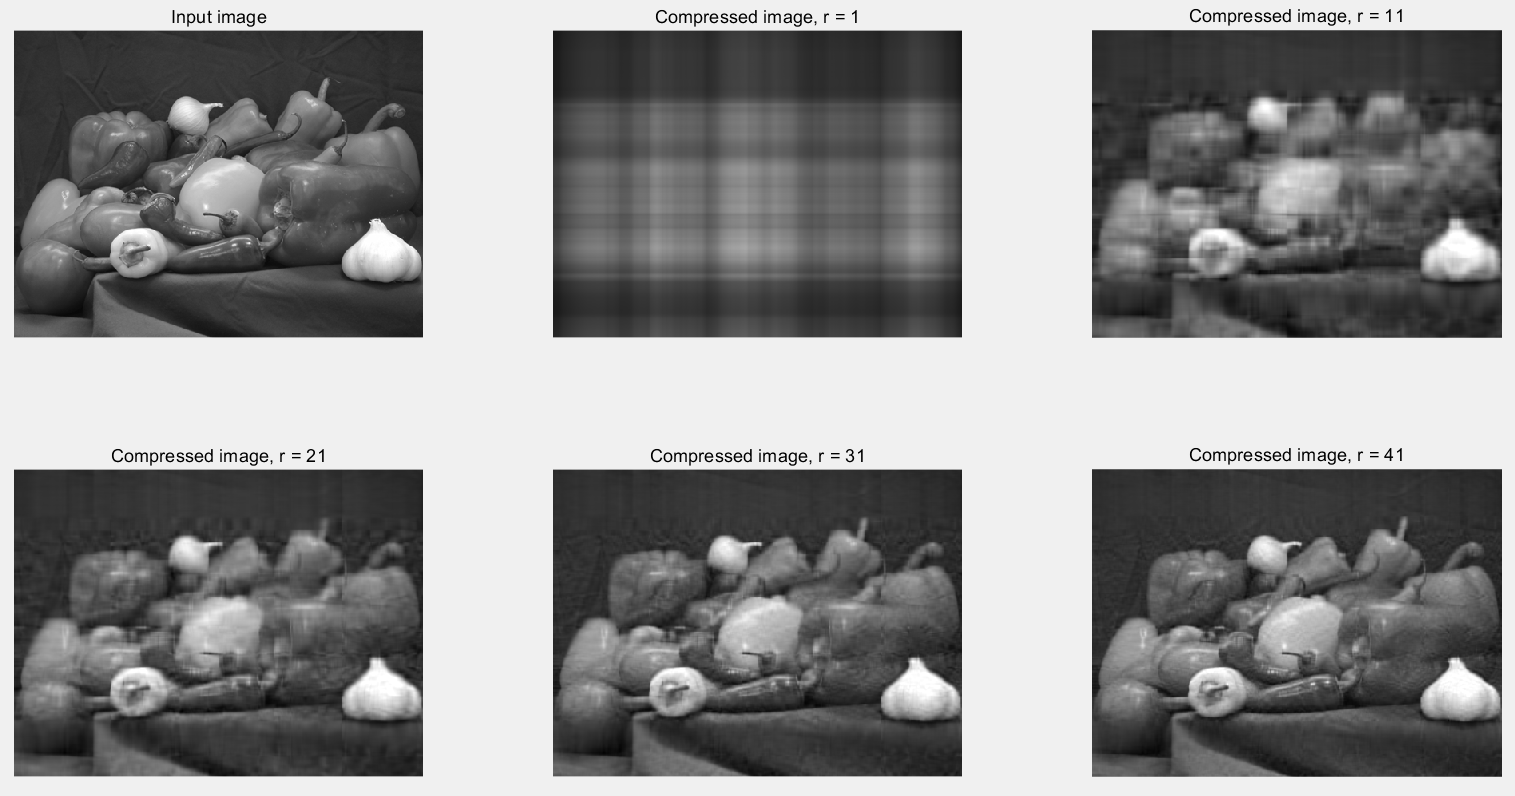
\includegraphics[scale=0.5]{Result_Gray.png}
        \caption{使用SVD分解压缩灰度图像peppers.png的结果}
        \label{figure:gray}
    \end{figure}
    
    考察原图像矩阵和各压缩图像的差异，计算重构误差和压缩率，如表2、3所示。
    \begin{table}[h]
    \centering
    \begin{minipage}[t]{0.45\textwidth}
        \centering
        \begin{tabular}{|l|l|}
        \hline
        r  & 重构误差   \\ \hline
        1  & 7070.212861 \\ \hline
        11 & 2120.128099 \\ \hline
        21 & 1330.170652 \\ \hline
        31 & 983.756099  \\ \hline
        41 & 799.764979  \\ \hline
        \end{tabular}
        \captionof{table}{灰度图像压缩前后矩阵差的二范数}
        \label{tab:table1}
    \end{minipage}
    \hfill % 水平填充，确保两个表格并排
    \begin{minipage}[t]{0.45\textwidth}
        \centering
        \begin{tabular}{|l|l|l|}
        \hline
        r  & 文件大小(Byte) & 压缩率 \\ \hline
        1  & 38,552 & 43.2\% \\ \hline
        11 & 62,432 & 70.0\% \\ \hline
        21 & 70,421 & 79.0\% \\ \hline
        31 & 74,571 & 83.6\% \\ \hline
        41 & 78,031 & 87.5\% \\ \hline
        \end{tabular}
        \captionof{table}{灰度图像的压缩率，原文件大小为 89,147 字节}
        \label{tab:table2}
    \end{minipage}
    \end{table}
    
    注意到随着r增大，重构误差减小，压缩图像更接近原图像；压缩率增大，压缩图像包含的信息越多。同时，r较大时，重构误差减小和压缩率增大的趋势较小，这是因为奇异值系数较小的项包含的信息较少导致的。
    
    \subsection{RGB图像的SVD压缩}
    采用RGB图像peppers.png，图像尺寸为384*512，利用SVD分解分别取\(r = 1, r = 11, r = 21, r = 31, r = 41\)，效果如图2。
    \begin{figure}[h]
        \centering %居中
        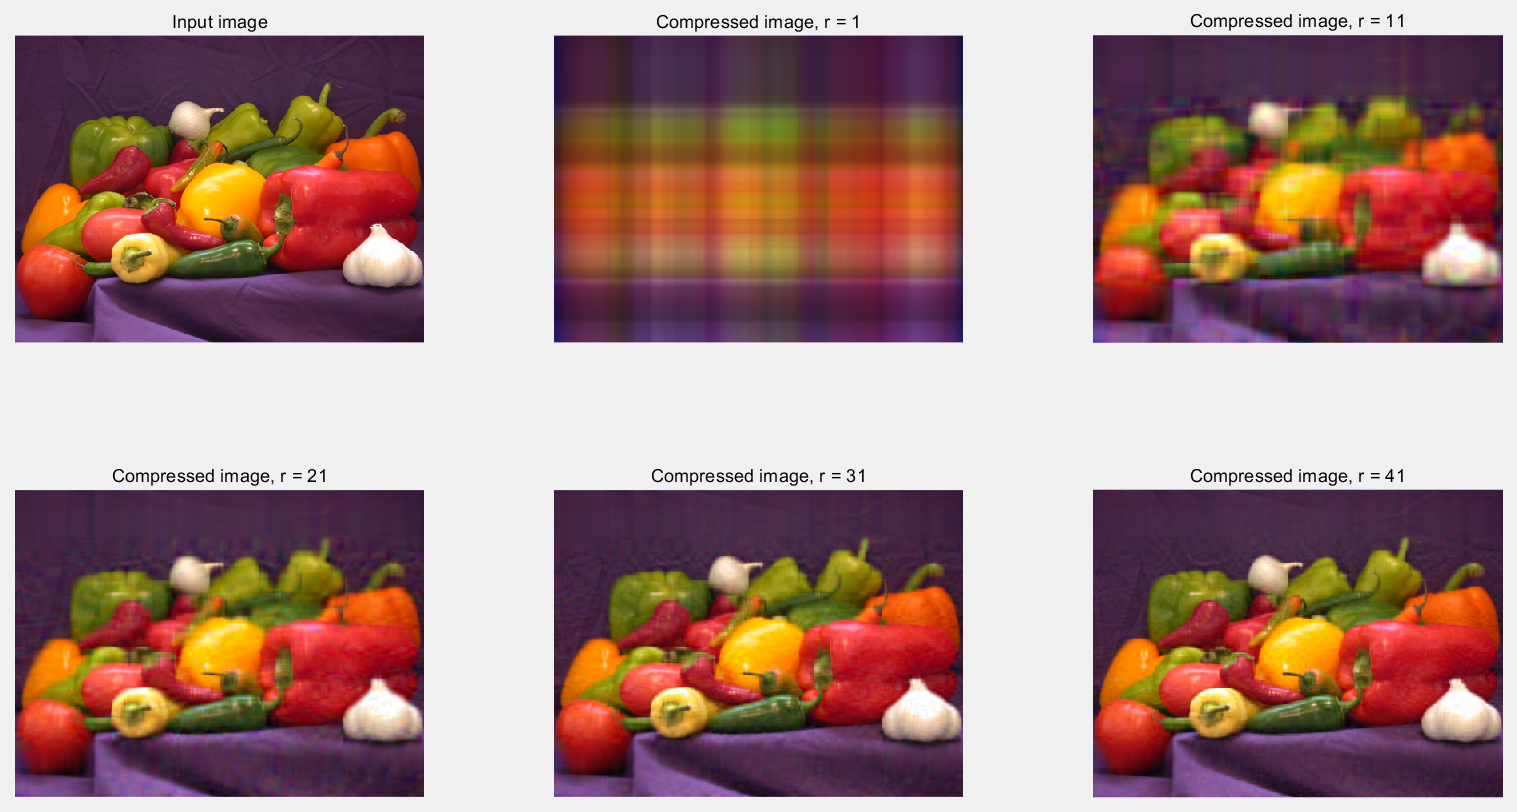
\includegraphics[scale=0.4]{Result_RGB.png}
        \caption{使用SVD分解压缩RGB图像peppers.png的结果}
        \label{figure:RGB}
    \end{figure}
    
    考察原图像矩阵和各压缩图像的差异，可以计算RGB三个通道的重构误差和压缩率，如表4、5所示。
    \begin{table}[h]
    \centering
    \begin{minipage}[t]{0.45\textwidth}
        \centering
        \begin{tabular}{|l|l|l|l|}
        \hline
        r  & 通道R & 通道G & 通道B \\ \hline
        1  & 8888.541552 & 8053.838560 & 6491.195570 \\ \hline
        11 & 2517.451336 & 2331.268616 & 2188.893316 \\ \hline
        21 & 1570.593824 & 1462.019859 & 1382.009425 \\ \hline
        31 & 1159.392304 & 1091.176497 & 1054.840436 \\ \hline
        41 & 922.474342  & 880.748346  & 876.602265  \\ \hline
        \end{tabular}
        \captionof{table}{RGB图像压缩前后各通道矩阵差的二范数}
        \label{tab:table3}
    \end{minipage}
    \hfill % 水平填充，确保两个表格并排
    \begin{minipage}[t]{0.45\textwidth}
        \centering
        \begin{tabular}{|l|l|l|}
        \hline
        r  & 文件大小 & 压缩率 \\ \hline
        1  & 130,562 & 45.4\% \\ \hline
        11 & 198,190 & 68.9\% \\ \hline
        21 & 219,782 & 76.4\% \\ \hline
        31 & 232,573 & 80.8\% \\ \hline
        41 & 242,733 & 84.4\% \\ \hline
        \end{tabular}
        \captionof{table}{RGB图像的压缩率，原文件大小为 287,677 字节}
        \label{tab:table4}
    \end{minipage}
    \end{table}

    随着r增大，各通道的重构误差和压缩率与灰度图像情况下的趋势保持一致，即重构误差减小，压缩率增大，趋势均减慢。

 \setcounter{section}{8}
\section*{\centerline{八、结论}}
    本报告介绍了基于SVD分解的图像压缩方法，描述了矩阵SVD分解的原理，并在MATLAB环境下针对灰度图像和RGB图像完成了代码实现，将其应用于示例图像的压缩，发现随着阶数r增大，图像矩阵表现出重构误差减小和压缩率增加的趋势，且趋势逐渐减慢。
    
 \setcounter{section}{9}
\section*{\centerline{九、问题}}
    通过对图像矩阵的SVD分解，可以有效地提取出图像的关键信息并压缩，但这一算法的缺点在于缺乏解释性，即SVD分解得到的矩阵中缺乏对关键部分的具体描述，导致用户并不知道图像的关键信息具体包含在哪些部分中。为解决这个问题，可以考虑引入图像识别算法（如图像卷积），进而显式地表示出关键信息的分布。
    
    此外，完整的SVD分解复杂度较高，对于较大的图像需要较多的时间成本，需要通过优化截断策略，如通过实验对比确定合适的\(r\)值等。
    
    同时，对于彩色图像，简单的分通道压缩没有关注各通道间的相关性，在实际任务中，需要通过各通道间的对比分析确定具体的压缩策略。
    
\bibliographystyle{ieeetr}
\bibliography{refer}

\end{document} 